\documentclass{beamer}
% \usepackage{animate}
\usepackage{multimedia}
\usepackage[english,russian]{babel}

\usepackage{pgfpages}
\setbeameroption{show notes on second screen}
%https://tug.ctan.org/macros/latex/contrib/beamer/doc/beameruserguide.pdf

\usepackage[T2A]{fontenc}
\usepackage[utf8]{inputenc}

\setbeamertemplate{caption}[numbered]

\usetheme{CambridgeUS}
\usecolortheme{dolphin}


\title[Построение изображений]{Процесс построения изображения}
\author[Быковских Д.А.]{Быковских Дмитрий Александрович}
\date{14.09.2024}

\begin{document}
\begin{frame}
	\titlepage
\end{frame}

%\section{Обзор}
\begin{frame}{Содержание}
	\begin{itemize}
		\item
		      Программные средства
		      %Спецификации и графические библиотеки
		\item
		      Процесс построения изображения
		\item
		      Модель графического конвейера
	\end{itemize}
\end{frame}

\section{Программные средства}
\begin{frame}{Терминология}
	{\scriptsize

		\textbf{Спецификация (стандарт, API)} --- документированные наборы правил, рекомендаций и параметров, определяющие способы взаимодействия, описание, единое понимание и совместимость между аппаратной и программной частями.

		\textbf{Драйвер (видеодрайвер)} --- программный интерфейс между операционной системой и графическим аппаратным обеспечением компьютера или устройства.
		%Графический драйвер выполняет важную роль в управлении и координации графическими функциями, такими как отображение изображений, обработка графики и управление монитором. Он обеспечивает абстракцию между аппаратурой и приложениями, позволяя программам использовать графические возможности устройства без необходимости знания специфических деталей аппаратной реализации.

		\textbf{Графическая библиотека} --- набор программных инструментов, функций и ресурсов, предназначенных для упрощения создания графических элементов в компьютерных приложениях.
		%Графические библиотеки предоставляют разработчикам доступ к базовым операциям рисования, управлению окнами, обработке ввода и другим визуальным компонентам.

		\textbf{Графический фреймворк} --- комплексная структура, предоставляющая базовую архитектуру и инструменты для разработки графических приложений.
		%В отличие от графических библиотек, фреймворки предоставляют более высокоуровневую абстракцию, объединяя не только графические, но и другие компоненты, такие как управление событиями, многозадачность и др.

		\textbf{Графический движок} --- программное обеспечение, которое предоставляет инфраструктуру и инструменты для разработки интерактивных графических приложений, игр и визуальных симуляций.
		%Графические движки обычно включают в себя готовые решения для управления графикой, физикой, анимацией, освещением и другими аспектами визуализации.

		\textbf{Графические редакторы} --- программное обеспечение, предназначенное для создания, редактирования и манипулирования графическими изображениями, включая различные эффекты, анимацию и многое другое.
		%Графические редакторы могут быть ориентированы на векторную или растровую графику, обеспечивая пользователю инструменты для рисования, изменения цветов, добавления эффектов и других операций над изображением.

		\textbf{Графический профилировщик} --- программное обеспечение, используемое для анализа и оптимизации производительности графических приложений или систем.
		%Графический профилировщик собирает данные о времени выполнения, использовании ресурсов (например, CPU и GPU), вызовах функций и других аспектах работы с графикой. Эти данные помогают разработчикам и инженерам идентифицировать узкие места, проблемы с производительностью и оптимизировать код или конфигурацию, чтобы обеспечить более плавное и эффективное взаимодействие графических приложений с аппаратурой и операционной системой.

		\textbf{GPU benchmark (бенчмарк графического процессора)} --- методика тестирования и оценки производительности графического процессора, которая позволяет измерить его способность обрабатывать графику и выполнение вычислительных задач.
		%В ходе GPU бенчмарка используются специально разработанные тестовые сцены или наборы задач, которые загружают графический процессор различными видами нагрузки, включая визуализацию 3D-графики, обработку текстур, вычисления с плавающей точкой и другие графические задачи. Результаты бенчмарка позволяют оценить производительность GPU, сравнить его с другими моделями или системами, а также определить, какие виды задач выполняются наиболее эффективно, что может быть полезно при выборе аппаратного обеспечения для конкретных целей.
	}

	\note{
		Графическое API (Application Programming Interface) — это набор интерфейсов и функций, предоставляемых операционной системой или программной средой, который позволяет программам взаимодействовать с аппаратным обеспечением для рендеринга графики. Графические API позволяют разработчикам управлять отображением 2D- и 3D-графики на экране, взаимодействовать с графическим процессором (GPU), управлять ресурсами (например, текстурами, шейдерами) и другими элементами графики.
	}
\end{frame}

\begin{frame}{Спецификации (API) и графические библиотеки}
	{\small
		\textbf{OpenGL (1992, Silicon Graphics)} \\
		Открытая кросс-платформенная спецификация для работы с 2D и 3D графикой

		\textbf{Mesa (1995, Brian Paul)} \\
		Свободная реализация графических API OpenGL (позже Vulkan и др.) с открытым исходным кодом

		\textbf{DirectX (1995, Microsoft)} \\
		Пакет графических API для работы с играми и мультимедийными приложениями на платформе Windows

		\textbf{WebGL (2011,	Khronos Group)} \\
		Графический API для веб-браузеров

		\textbf{Mantle (2013, AMD)} \\
		Спецификация низкоуровневого API

		\textbf{Vulkan (2016, Khronos Group)} \\
		Низкоуровневый (требует явного управления памятью и ресурсами) высокопроизводительный кроссплатформенный API для работы с 2D и 3D графикой
	}



\end{frame}

\begin{frame}{MESA}
	MESA --- это открытый проект, который предоставляет реализацию различных графических API (таких как OpenGL, OpenGL ES, Vulkan, OpenCL и др.) для Linux и других операционных систем с открытым исходным кодом.

	MESA поддерживает реализацию OpenGL для устройств, разработанных Intel, AMD, NVIDIA, Qualcomm и др., включая виртуальные графические процессоры VMware и VirGL.
	Также есть несколько программных рендереров: Softpipe (драйвер Gallium) и LLVMpipe (высокоскоростной растеризатор на основе LLVM/JIT).

	\note{
		Проект начал разрабатывать Брайн Пол в 1993. Основная цель заключалась в реализация OpenGL подобной IRIS GL.

		Первая версия вышла в 1995 с разрешения SGI. Названа в честь языка программирования MESA.

		https://docs.mesa3d.org/history.html
		% 	% https://www.mesa3d.org/

	}

\end{frame}


\begin{frame}{Структура современной графической библиотеки}
	\textbf{Графический движок} (движок рендеринга 2-х или 3-х мерной КГ)

	%Порядок приоритетов поменять

	\begin{itemize}
		\item
		      Должны работать в реальном времени
		\item
		      Поддержка шейдеров
	\end{itemize}

	\textbf{Анимация}
	\begin{itemize}
		\item
		      Кинематика(компьютерный фильм)
	\end{itemize}

	\textbf{Физический движок }(физика)
	\begin{itemize}
		\item
		      Динамика жидкости, газа, взаимодействия тел и т.д.
	\end{itemize}

	\textbf{Игровой ИИ} (game artificial intelligence)
	\begin{itemize}
		\item
		      Боты (bots), моды (mods) и неигровые персонажи (non-player characters)
	\end{itemize}

	\textbf{Звук, система скриптов (система I/O), сетевой интерфейс} и т.д.
\end{frame}

\begin{frame}{Распределение вычислений между CPU и GPU}{Central and Graphical Processor Unit}
	%GPU а термин не ввел.
	\begin{figure}
		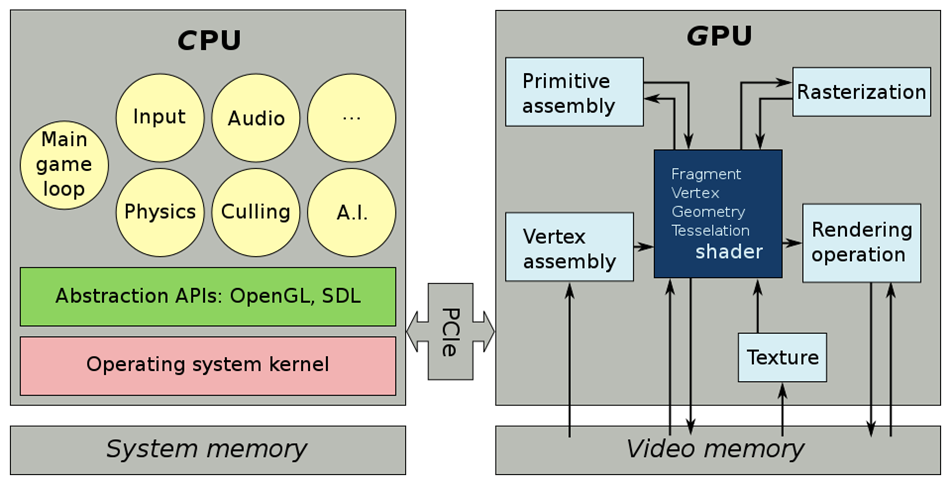
\includegraphics[width=0.95\textwidth]{images/Calculation_distribution_scheme.png}
		\caption {Принципиальная схема распределения вычислений}
	\end{figure}


	\note{
		\begin{figure}
			\href{https://jagatplay.com/2024/03/news/sony-akan-umumkan-ghost-of-tsushima-versi-pc-minggu-ini/}{
				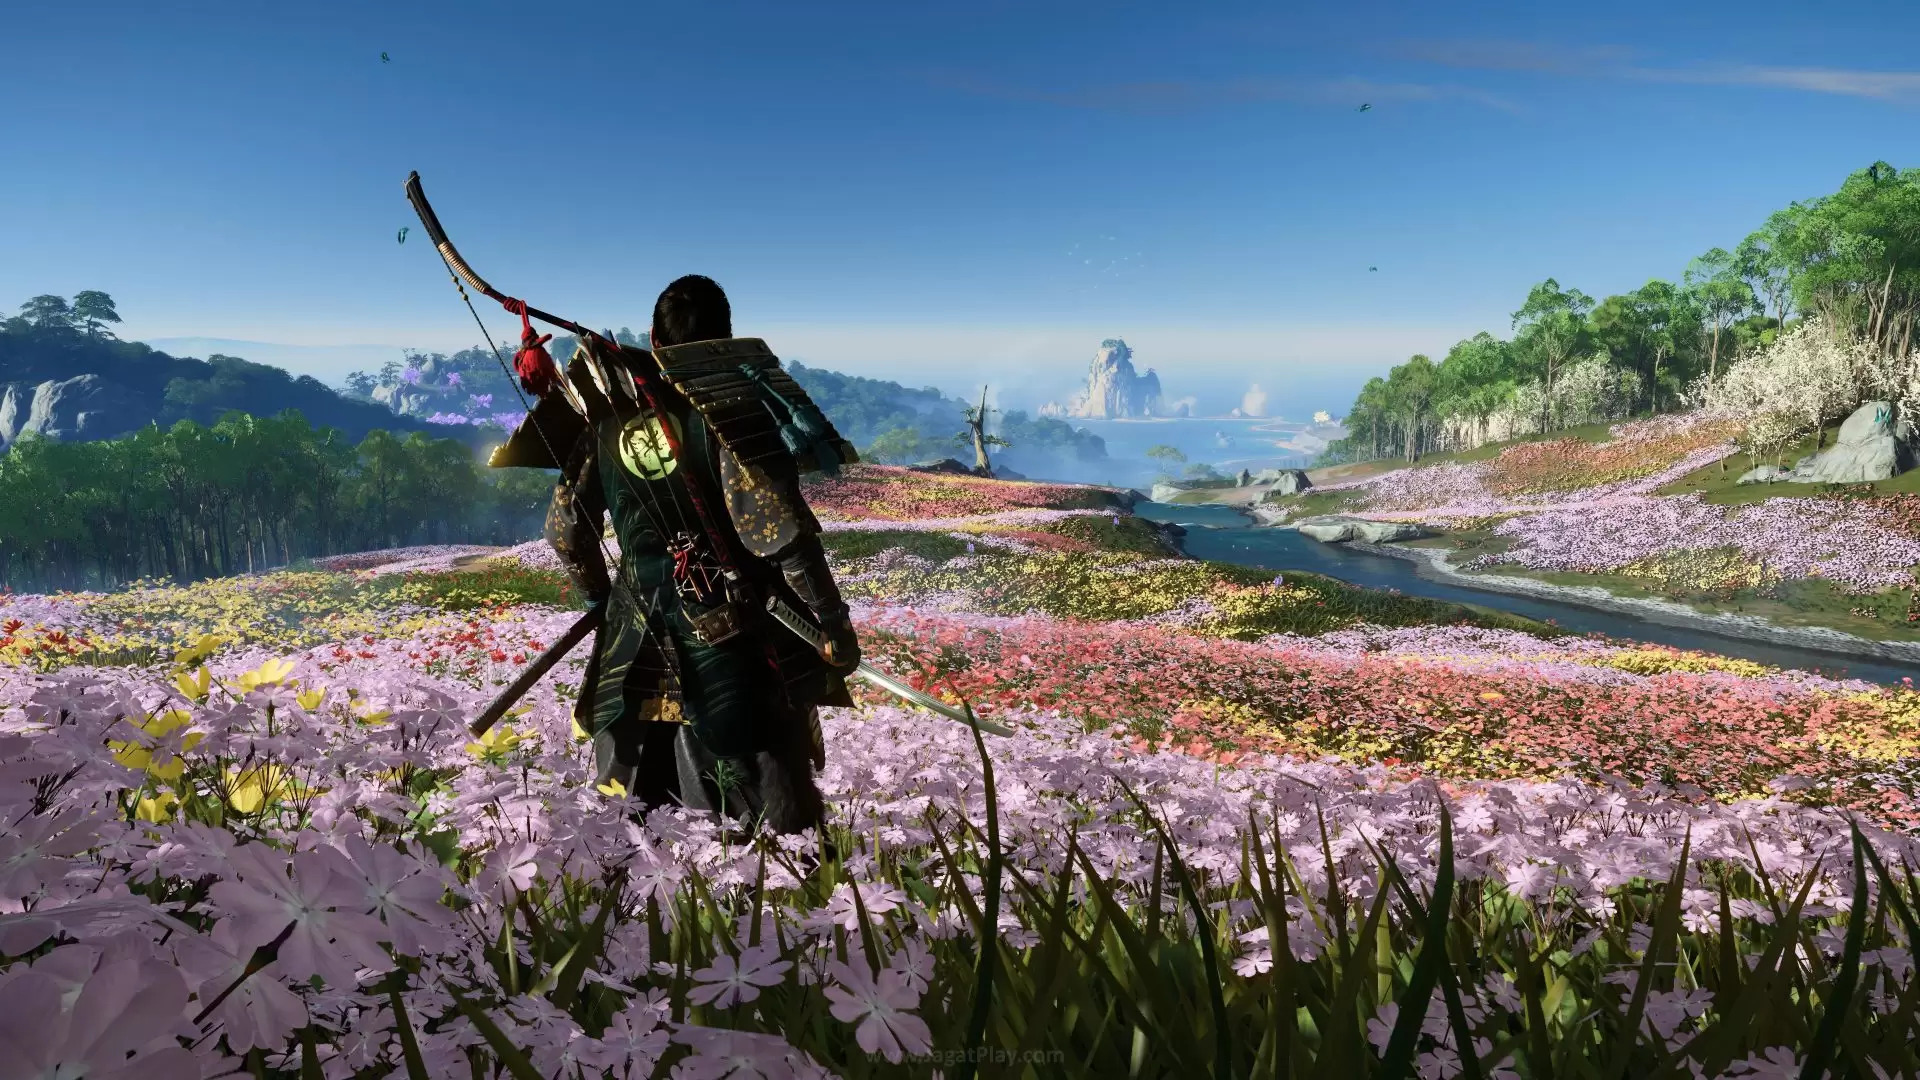
\includegraphics[width=0.8\textwidth]{images/Ghost_of_Tsushima.jpeg}}
			\caption{Ghost of Tsushima (2024, Призрак Цусимы)}
		\end{figure}

	}
\end{frame}

\section{Процесс построения изображения}

\begin{frame}{Растровая графика}
	\begin{figure}
		\href{https://creativeyatra.com/news/windows-ends-journey-ms-paint-three-decades}{
			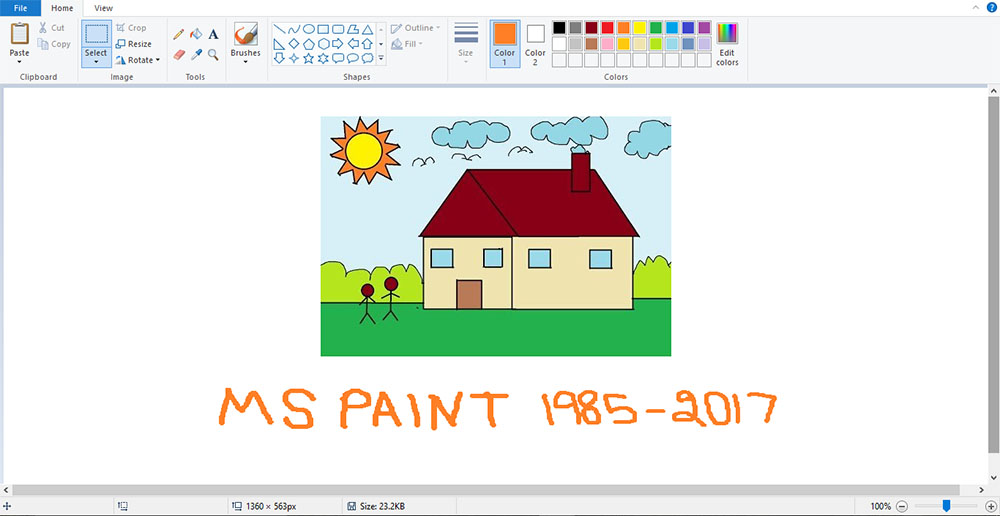
\includegraphics[width=0.9\textwidth]{images/MS_Paint.jpg}}
		\caption{MS Paint}
	\end{figure}

	\note{
		Растровая графика (bitmap или pixel-based) представляет изображение в виде массива пикселей.
		Каждый пиксель хранит информацию о цвете, расположенные в опредленном порядке формируют изображение.

		Качество изображения зависит от количества пикселей.
		Чем выше разрешение (количество пикселей на единицу площади), тем детализированнее изображение.
	}
\end{frame}

\begin{frame}{Векторная графика}
	\begin{figure}
		\href{https://www.gimp.org/}{
			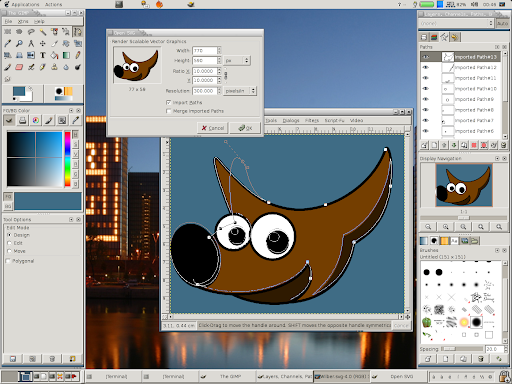
\includegraphics[width=0.7\textwidth]{images/GIMP.png}}
		\caption{GIMP}
	\end{figure}

	\note{
		Векторная графика представляет изображение соостоящее из примитвов и/или математических объектов (линии, точки, треугольники, кривые, поверхности и др.).
		Эти объекты описываются с помощью набора параметров и/или уравнений, что позволяет бесконечно масштабировать изображение без потери качества.
	}
\end{frame}

\begin{frame}{Воксельная графика}
	\begin{figure}
		\href{https://ephtracy.github.io}{
			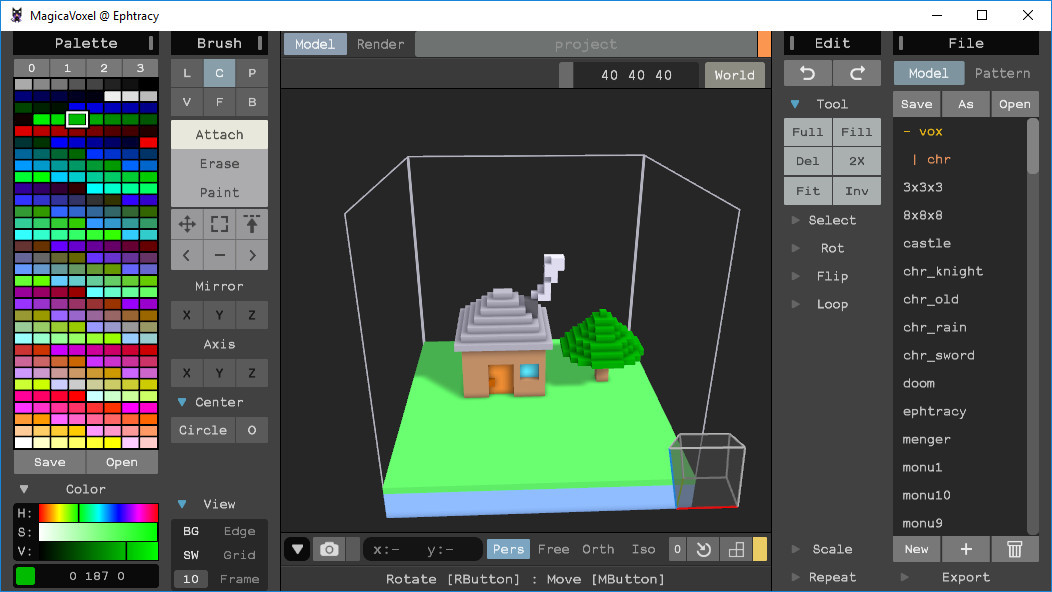
\includegraphics[width=0.9\textwidth]{images/MagicaVoxel.jpg}}
		\caption{Виды преобразований и системы координат}
	\end{figure}

	\note{
		Воксельная графика --- это трехмерный аналог растровой графики, где изображение состоит из объёмных пикселей, называемых вокселями (volume elements, объемные элементы).
		Воксели представляют собой кубические блоки, которые формируют объёмные объекты в 3D-пространстве.
	}
\end{frame}

\begin{frame}{Процесс построения изображения}
	\begin{figure}
		\href{https://learnopengl.com/Getting-started/Coordinate-Systems}{
			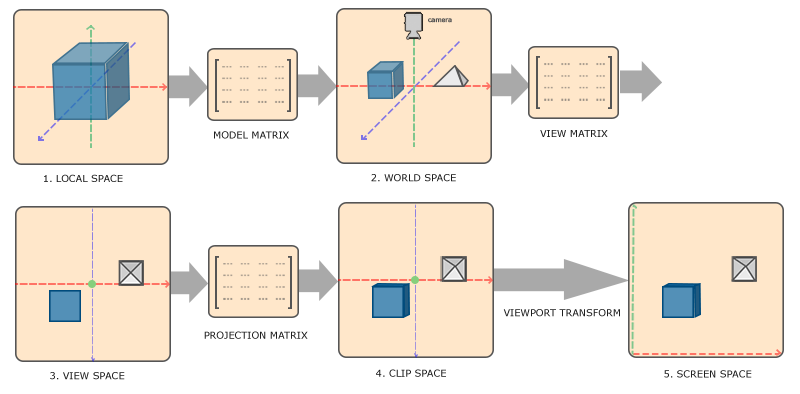
\includegraphics[width=\textwidth]{images/Coordinate_systems.png}}
		\caption{Виды преобразований и системы координат}
	\end{figure}

	\note{
	\hfill Локальные координаты (ЛК)
	\\ 
	\hfill (координаты модели)

	Геометрические преобразования
	 
	\hfill Мировые координаты (МК)
	\\ 
	\hfill (координаты модели в сцене)

	Преобразование наблюдения

	\hfill Координаты наблюдения (КН)

	Преобразование проецирования,
	\\
	включая нормирование и отсечение

	\hfill Нормированные координаты (НК)

	Преобразование поля просмотра, 
	\\
	включая растеризацию

	\hfill Координаты устройства (КУ)
	}
\end{frame}

\begin{frame}{Процесс построения изображения}
	\begin{figure}
		\href{https://www.researchgate.net/figure/Outline-of-the-graphics-pipeline_fig1_281810652}{
			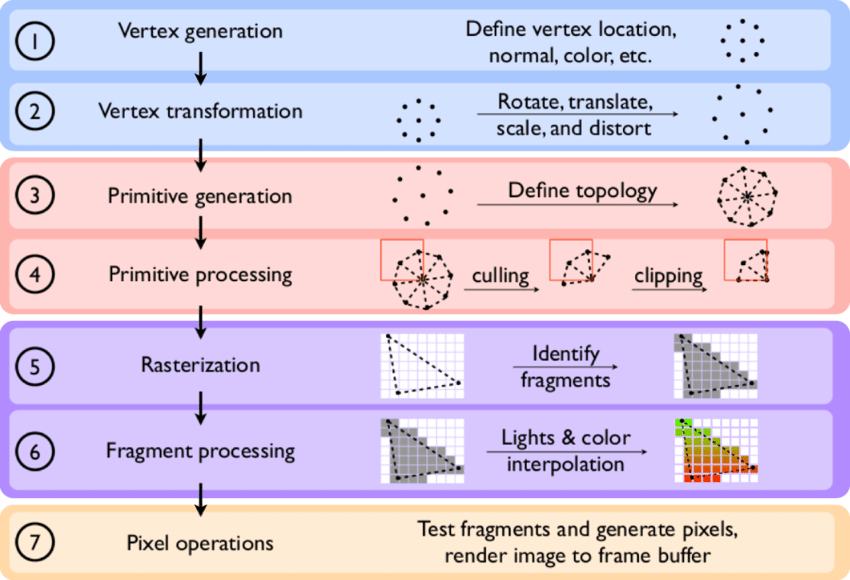
\includegraphics[width=0.75\textwidth]{images/Outline-of-the-graphics-pipeline.png}}
		\caption{Схема графического конвейера}
	\end{figure}
\end{frame}

\begin{frame}{Конвейер рисования в OpenGL}{}
	\begin{figure}
		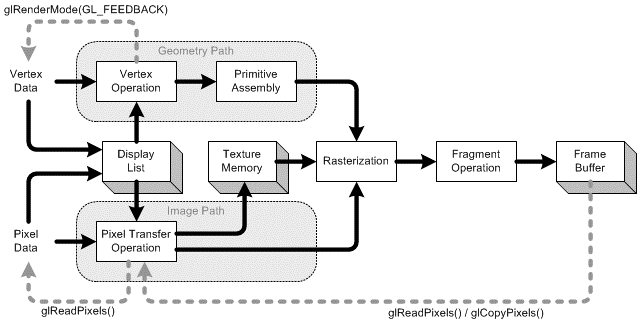
\includegraphics[width=0.95\textwidth]{images/OpenGL_graphics_pipeline.png}
		\caption {Принципиальная схема распределения вычислений}
	\end{figure}
\end{frame}

\section{Vодель графического конвейера}

\begin{frame}{Упрощенная схема графического конвейера}{Shaders}
	\begin{columns}
		\begin{column}{0.5\textwidth}
			\begin{figure}
				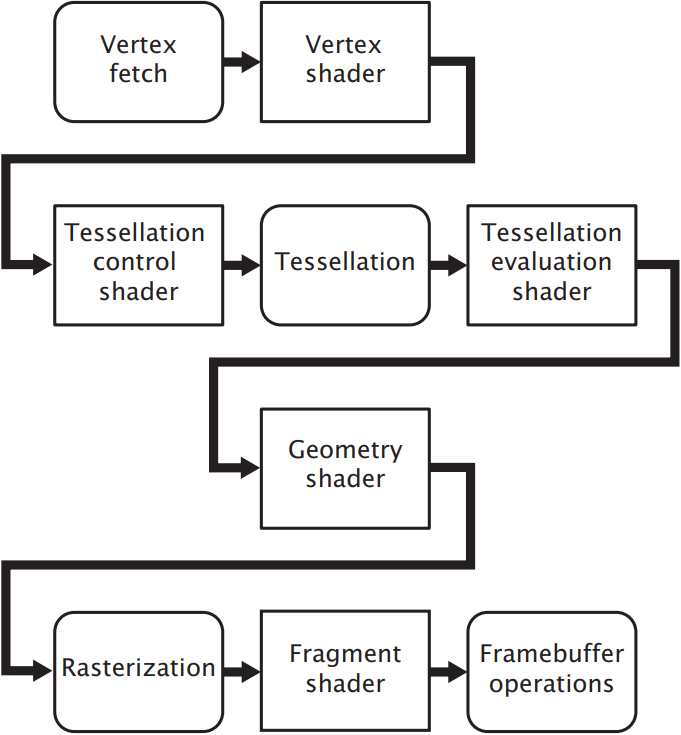
\includegraphics[width=0.9\textwidth]{images/Simplified_model_of_the_graphics_pipeline.png}
				\caption {Порядок вычисления шейдеров}
			\end{figure}
		\end{column}
		\begin{column}{0.5\textwidth}

			{\footnotesize

			Загрузка данных

			{\hfill Вершина (vertices)}

			\textbf{Вершинный шейдер}

			{\hfill Группа вершин (primitives/patches)}

			\textbf{Шейдер управление тесселяцией}

			Тесселяция

			\textbf{Шейдер определяющий тесселяции}

			{\hfill Примитивы (primitives)}

			\textbf{Геометрический шейдер}

			{\hfill Примитивы (primitives)}

			Растеризация и интерполяция

			{\hfill Пиксели (fragments)}

			\textbf{Пиксельный (фрагментный) шейдер}

			{\hfill Пиксели (fragments)}

			Операции с буферами кадров

			{\hfill Пиксели (Pixels)}
			}
		\end{column}
	\end{columns}


\end{frame}


\begin{frame}{Упрощенная модель графического конвейера}{OpenGL API}
	\begin{figure}
		\href{https://registry.khronos.org/OpenGL/specs/gl/glspec46.core.pdf}{
			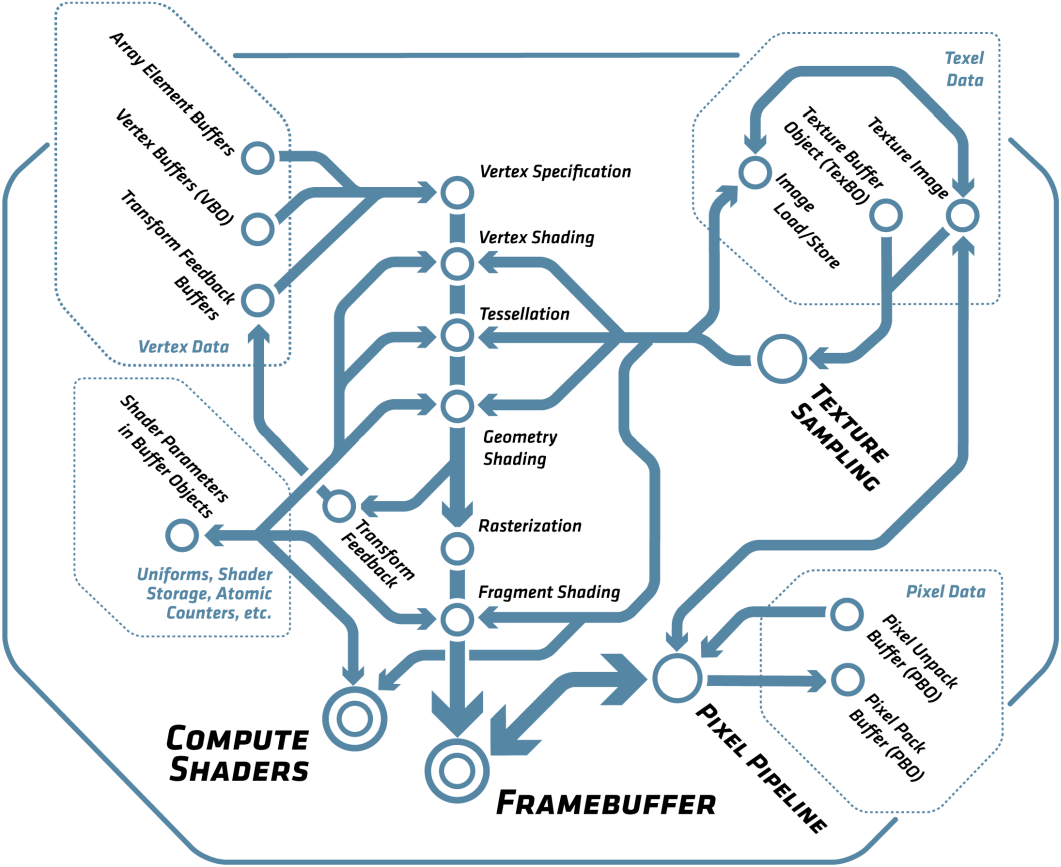
\includegraphics[width=0.6\textwidth]{images/OpenGL_specification_graphics_pipeline.png}}
		\caption {Принципиальная схема распределения вычислений}
	\end{figure}

	\note {

	}
\end{frame}

\begin{frame}{Упрощенная модель графического конвейера}{Vulkan API}
	\begin{figure}
		\href{https://docs.vulkan.org/spec/latest/chapters/pipelines.html}{
			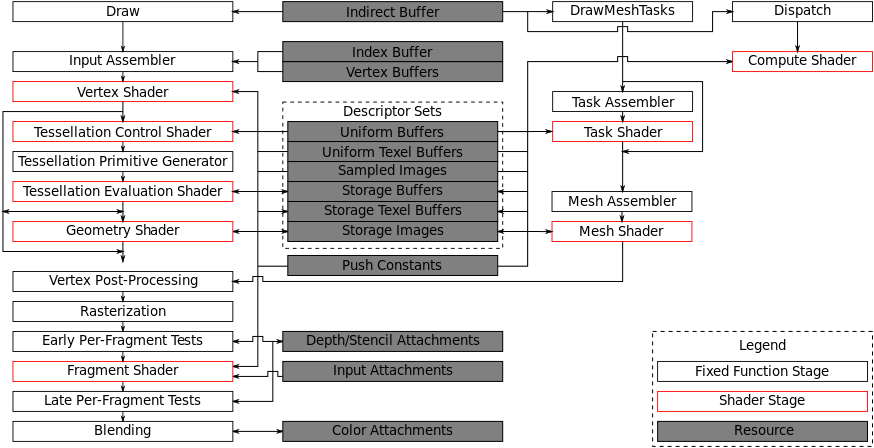
\includegraphics[width=0.95\textwidth]{images/Vulkan_pipelinemesh.png}}
		\caption {Блок-схема конвейера Vulkan API}
	\end{figure}

	\note {


	}
\end{frame}

\if 0
	\begin{columns}

		\begin{column}{0.5\textwidth}
			\begin{itemize}
				\item

			\end{itemize}
		\end{column}
		\begin{column}{0.5\textwidth}
			\begin{itemize}
				\item
			\end{itemize}
		\end{column}

	\end{columns}
\fi

\end{document}
